\documentclass[10pt]{beamer}

%\setbeameroption{show notes on second screen=right}

% -------------------- Theme --------------------
\usetheme{Madrid}
%\setbeamertemplate{navigation symbols}{}

\setbeamercovered{transparent}

% -------------------- Ahmedabad University Colors --------------------
\definecolor{AUred}{RGB}{128,18,20}      % Primary logo red
\definecolor{AUdark}{RGB}{160,160,160}    % Dark gray for text
\definecolor{AUlight}{RGB}{242,239,236} % Light background


\definecolor{arsenic}{rgb}{0.23, 0.27, 0.29}
\definecolor{bole}{rgb}{0.47, 0.27, 0.23}
\definecolor{brown(web)}{rgb}{0.65, 0.16, 0.16}
\definecolor{cadet}{rgb}{0.33, 0.41, 0.47}
\definecolor{cordovan}{rgb}{0.54, 0.25, 0.27}
\definecolor{daffodil}{rgb}{1.0, 1.0, 0.19}
\definecolor{brown(traditional)}{rgb}{0.59, 0.29, 0.0}
\colorlet{slidebg}{white}
\colorlet{boxbg}{blue!6}
\colorlet{textlight}{black}
\colorlet{netblue}{blue!65!black}
\colorlet{embedgreen}{green!45!black}
\colorlet{SharedWeight}{red!60!black}
\colorlet{distamber}{orange!80!black}

% -------------------- Apply Colors --------------------
\setbeamercolor{structure}{fg=AUred}

\setbeamercolor{title}{fg=AUlight}
\setbeamercolor{subtitle}{fg=AUdark}

\setbeamercolor{frametitle}{fg=AUdark, bg=AUred}
\setbeamercolor{framesubtitle}{fg=AUlight}
\setbeamercolor{section in head/foot}{fg=AUlight, bg=AUred}

\setbeamercolor{block title}{fg=AUlight, bg=AUred}
\setbeamercolor{block body}{fg=black, bg=AUlight}

\setbeamercolor{item}{fg=AUred}
\setbeamercolor{subitem}{fg=AUred}

\setbeamercolor{footline}{fg=white, bg=AUred}

% -------------------- Frame Title Fonts --------------------
\setbeamerfont{frametitle}{size=\small,series=\bfseries}
\setbeamerfont{framesubtitle}{size=\large}

\setbeamerfont{caption}{size=\scriptsize}


% -------------------- Packages --------------------
\usepackage{amsmath}
\usepackage{amsfonts}
\usepackage{graphicx}
\usepackage{booktabs}
\usepackage{nameref}
\usepackage{natbib}
\usepackage{tikz}
\usepackage{amssymb}    % for \checkmark
\usepackage{multirow}


\usetikzlibrary{calc, positioning, arrows.meta, fit, backgrounds, shapes.geometric}
\usepackage{xcolor}
\bibliographystyle{plainnat}





% Local colors (already defined in preamble via color_fix — kept here for safety)
\providecolor{netblue}{named}{blue}
\colorlet{SBlue}{blue!70!black}
\colorlet{SGreen}{green!50!black}
\colorlet{SRed}{red!60!black}
\colorlet{SAmber}{orange!85!black}
\colorlet{SBlueBg}{blue!9}
\colorlet{SGreenBg}{green!9}
\colorlet{SRedBg}{red!8}
\colorlet{SAmberBg}{orange!10}
\colorlet{SGrayBg}{black!5}



% -------------------- Title Info --------------------
\title[Online Tracker for Small Object Detection]{Improve performance of existing online trackers for small object detection}
\subtitle{UAV videos}

\author[Sheth A., Parekh M., Thanki K., Riddhi B.]{
	Team Name: \textbf{The Convolutioners} \\
	\textbf{Aagam Sheth} (AU2544006) \\	
	\textbf{Mahima Parekh} (AU2544003) \\
	\textbf{Khevan Thanki} (AU23L20002) \\
	\textbf{Riddhi Bhargava} (AU2220028)
}

\institute[]{
	Instructor Name: \textbf{Prof. Mehul Raval} \\
	Assigned TA: \textbf{Daksh D. Shah} \\
	School of Engineering and Applied Science \\
	\vspace{0.2cm}
	\includegraphics[width=3cm]{"/home/aagamsheth/Documents/Education/Ahmedabad University/media/au_logo.png"}
}

\date{\today}

% -------------------- Logo on Each Slide --------------------
\addtobeamertemplate{frametitle}{}{
	\hfill
	\raisebox{0.7cm}[0pt][0pt]{\includegraphics[height=0.8cm,keepaspectratio]{"/home/aagamsheth/Documents/Education/Ahmedabad University/media/au_logo_dark.png"}}
}


% -------------------- Document --------------------
\begin{document}
	
	% -------------------- Title Slide --------------------
	{
		\logo{}
		\begin{frame}
			\titlepage
		\end{frame}
	}
	
	\begin{frame}{Background}{Problem Statement}	
		\begin{itemize}
			\item \textbf{Challenges} faced in detection:
				\begin{itemize}
					\item Tiny objects $\rightarrow$ few pixels
					\item Clutter, motion blur, scale variation
					\item Unreliable detections
				\end{itemize}
		\end{itemize}
		
		\vspace{0.25cm}
		\begin{itemize}
			\item Unreliable detections lead to:
			\begin{itemize}
				\item Missed detections
				\item Identity switches
				\item Poor tracking performance
			\end{itemize}
		\end{itemize}
		
		\vspace{0.5cm}
		\begin{block}{Research Gap}
			Existing methods are not optimized for small object detection in UAV scenarios, resulting in poor detection quality and inconsistent identity association even with tiling and ReID.
		\end{block}
	\end{frame}

	\begin{frame}{Full pipeline of work}{Methodology Overview}
		\centering
		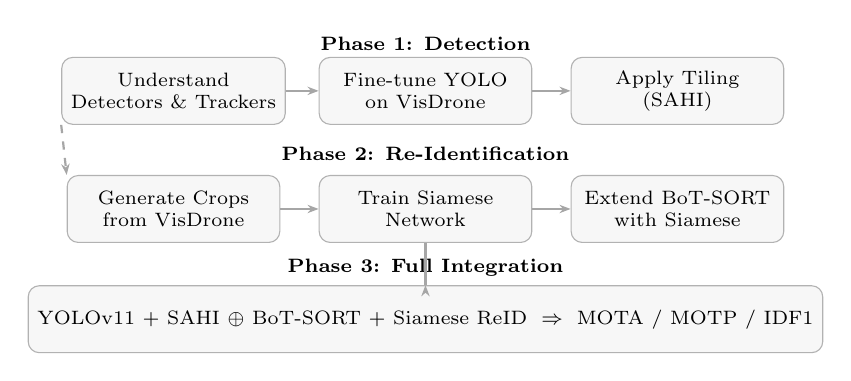
\begin{tikzpicture}[
			>=Stealth,
			box/.style={
				draw=black!30, fill=black!3, rounded corners=4pt,
				minimum width=2.7cm, minimum height=0.85cm,
				align=center, font=\scriptsize
			},
			arr/.style={-{Stealth[length=4pt]}, line width=0.8pt, color=black!35},
			]
			
			% ── Phase 1 ──────────────────────────────────────────────────────
			\node[font=\scriptsize\bfseries, draw=none] at (3.2, 2.3) {Phase 1: Detection};
			
			\node[box] (n1) at (0,   1.7) {Understand\\Detectors \& Trackers};
			\node[box] (n2) at (3.2, 1.7) {Fine-tune YOLO\\on VisDrone};
			\node[box] (n3) at (6.4, 1.7) {Apply Tiling\\(SAHI)};
			
			\draw[arr] (n1) -- (n2);
			\draw[arr] (n2) -- (n3);
			
			% ── Phase 2 ──────────────────────────────────────────────────────
			\node[font=\scriptsize\bfseries, draw=none] at (3.2, 0.9) {Phase 2: Re-Identification};
			
			\node[box] (p1) at (0,   0.2) {Generate Crops\\from VisDrone};
			\node[box] (p2) at (3.2, 0.2) {Train Siamese\\Network};
			\node[box] (p3) at (6.4, 0.2) {Extend BoT-SORT\\with Siamese};
			
			\draw[arr] (p1) -- (p2);
			\draw[arr] (p2) -- (p3);
			\draw[arr, dashed] (n1.south west) -- (p1.north west);
			
			% ── Phase 3 ──────────────────────────────────────────────────────
			\node[font=\scriptsize\bfseries, draw=none] at (3.2, -0.55) {Phase 3: Full Integration};
			
			\node[box, minimum width=9cm] (final) at (3.2, -1.2)
			{YOLOv11 + SAHI $\oplus$ BoT-SORT + Siamese ReID
				$\;\Rightarrow\;$ MOTA / MOTP / IDF1};
			
			\draw[arr] (p2.south) -- ++(0,-0.1) |- (final.north);
			
		\end{tikzpicture}
	\end{frame}
	
	\begin{frame}{Results}{Baseline Metrics}
		\footnotesize
		\definecolor{good}{RGB}{0,140,0}
		\definecolor{bad}{RGB}{200,0,0}
		
		\begin{table}
			\centering
			\begin{tabular}{lcccc}
				\toprule
				\textbf{Category} & \textbf{Metric} & \textbf{YOLOv8n (Siamese NW)} & \textbf{YOLO11 (FT)} & \textbf{YOLO11 + SAHI} \\
				\midrule
				
				Tracking 
				& MOTA & 12.9\% & 16.73\% & \textcolor{good}{17.28\% $\uparrow$} \\
				& IDF1 & 22.4\% & \textcolor{good}{49.02\%} & 48.79\% \\
				& HOTA & \textcolor{good}{26.0\%} & 21.24\% & -- \\
				
				\midrule
				Detection 
				& DetA & 14.2\% & \textcolor{good}{30.14\%} & -- \\
				
				\midrule
				Association 
				& AssA & \textcolor{good}{50.4\%} & 15.57\% & -- \\
				& IDP / IDR & \textcolor{good}{81.7 / 13.0} & -- & -- \\
				
				\midrule
				Localization 
				& MOTP & 22.2\% & 26.51\% & \textcolor{good}{26.01\%} \\
				
				\midrule
				Detection
				& Precision & \textcolor{good}{81.68\%} & -- & 61.12\% \\
				& Recall & 12.98\% & -- & \textcolor{good}{49.07\%} \\
				
				\midrule
				Efficiency 
				& FPS & \textcolor{good}{12.69} & 0.5 & 0.5 \\
				
				\bottomrule
			\end{tabular}
		\end{table}		
	\end{frame}
	
	
	\begin{frame}{Results}{Siamese Network Analysis}
		\footnotesize
		\centering
		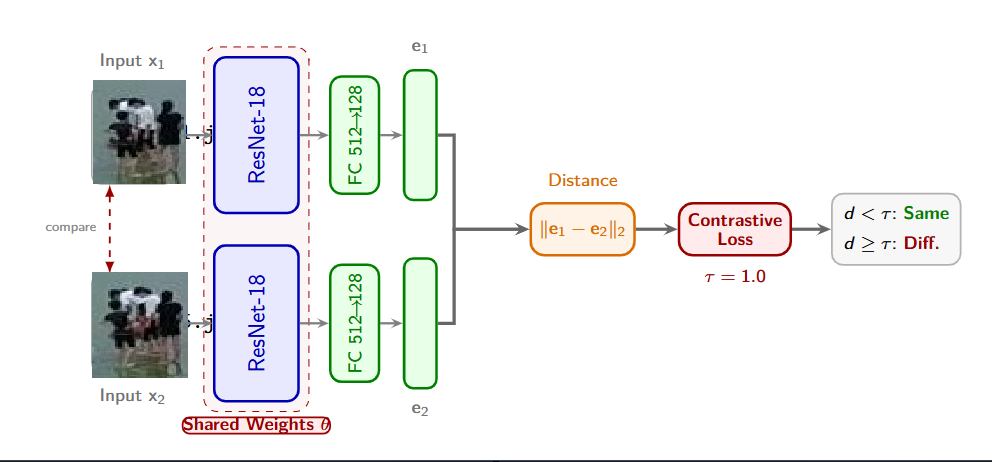
\includegraphics[width=\textwidth]{images/3.png}
	\end{frame}
	
	
	
	\begin{frame}{Results}{Siamese Network Analysis}
		\centering
		\scriptsize
		\textbf{Embedding Distance}
		\vspace{0.1cm}
		
		\begin{tabular}{lcc}
			\toprule
			Metric & Ep 1 & Ep 5 \\
			\midrule
			Same Obj & 0.48 & 0.26 \\
			Diff Obj & 1.15 & 1.04 \\
			\bottomrule
		\end{tabular}
		
		\vspace{0.3cm}
		
		\scriptsize
		\textbf{Training Performance}
		\vspace{0.15cm}
		
		\begin{tabular}{lccccc}
			\toprule
			Ep & Loss & Acc & Prec & Rec & F1 \\
			\midrule
			1 & 2.66 & 0.66 & 0.60 & 0.97 & 0.74 \\
			2 & 0.21 & 0.67 & 0.61 & 0.99 & 0.75 \\
			3 & 0.13 & 0.71 & 0.63 & 1.00 & 0.77 \\
			4 & 0.09 & \textbf{0.79} & 0.70 & 1.00 & \textbf{0.82} \\
			5 & \textbf{0.08} & 0.77 & 0.68 & 1.00 & 0.81 \\
			\bottomrule
		\end{tabular}
	\end{frame}
	
	
	\begin{frame}{Conclusions}{Future Scope}
		
		\small
		
		\begin{itemize}
			
			\item \textbf{Full Pipeline Integration} \\
			YOLO11 + SAHI $\rightarrow$ Siamese-enhanced BoT-SORT $\rightarrow$ end-to-end system evaluation
			
			\vspace{0.2cm}
			
			\item \textbf{Improve Detection \& Tracking} \\
			Compare advanced trackers: ByteTrack, OC-SORT, NV-SORT
			
			\vspace{0.2cm}
			
			\item \textbf{False Positive Reduction} \\
			NMS $\rightarrow$ Soft-NMS / Adaptive Thresholding $\rightarrow$ fewer duplicate detections
			
			\vspace{0.2cm}
			
			\item \textbf{Enhanced Re-Identification} \\
			\begin{itemize}
				\item Advanced loss functions
				\item Data augmentation for small objects
			\end{itemize}
			
			\vspace{0.2cm}
			
			\item \textbf{Evaluation on Diverse Datasets} \\
			VisDrone $\rightarrow$ DRASHTI $\rightarrow$ improved generalization
			
		\end{itemize}
		
	\end{frame}
	
	
	
	\begin{frame}{Appendix}{References}
		
		\footnotesize
		
		\begin{itemize}
			
			\item Xiao, Y. et al. (2025). \textit{UAV video vehicle detection: Benchmark and baseline}. IEEE TGRS.
			
			\item Wang, J. et al. (2021). \textit{Tiny object detection in aerial images}. ICPR.
			
			\item Liu, M. et al. (2020). \textit{UAV-YOLO: Small object detection from UAV perspective}. Sensors.
			
			\item Feng, F. et al. (2024). \textit{Improved YOLOv8 for small object detection in aerial imagery}. Journal of King Saud University.
			
		\end{itemize}
		
	\end{frame}
	
	
\end{document}